\chapter{引言}
\label{cha:intro}

\section{研究意义}
\label{sec:first}
视觉是人类感知世界最直接和重要的方法之一,光线通过眼睛、视网膜、大脑等器官的处理,最终形成我们所感知的图像~\cite{GonzalezDIP}。随着科技的发展,数码相机、摄像机等的出现使得数字图像和视频成为了人们日常生活中最常见的数字媒体之一。特别是随着近年来智能手机、移动互联网、社交网络的飞速发展和普及,人们随时随地都可以将眼前所见拍摄成图像或视频,并通过网络分享给自己在世界各地的亲朋好友。这些海量的数字图像和视频信息的处理已经成为计算机科学等领域重要的研究内容。当前,图像和视频处理已经从传统的基于像素的处理,例如图像去噪、图像增强、图像压缩等,逐步转移到基于内容的处理,例如基于内容的编辑、基于内容的检索等~\cite{CMM12THU}。根据经验,我们在观察图像或视频时,一般会将注意力集中在某些感兴趣区域,例如,在观看电影时我们的视觉注意力主要集中在主要角色身上。生物学家和心理学家通过研究和实验证实,人类的视觉系统只对图像的某些局部进行处理,而对其余部分几乎完全忽略~\cite{treisman1980a,Koch1985Shifts}。一般将人类视觉系统感兴趣的这类对象称为前景对象或显著性对象(saliency objects);相反,图像中的另外一部分则称为背景。背景减除,或前景检测,是指将图像或视频中背景部分去除,从而使前景对象和背景对象分离的一种技术。例如,在图~\ref{fig:1}中,~\ref{fig:subfig1}中为输入图像,~\ref{fig:subfig2}中为背景减除技术提取的前景对象,其中用白色表示前景区域,黑色表示背景区域。\par
\begin{figure}[ht]
  \centering%
  \subcaptionbox{输入图像\label{fig:subfig1}} %标题的长度,超过则会换行,如下一个小图。
    {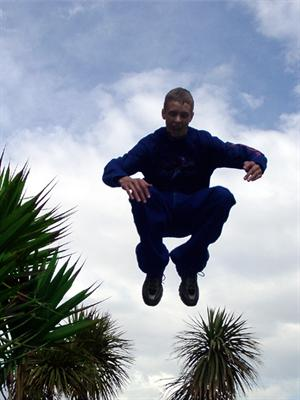
\includegraphics[width=0.3\textwidth]{ch1/0_0_818.jpg}}%
 \hspace{1em}%
  \subcaptionbox{背景减除结果,白色为前景,黑色为背景\label{fig:subfig2}}
      {
\includegraphics[width=0.3\textwidth]{ch1/0_0_818.png}}
  \caption{图像背景减除示例}
  \label{fig:1}
\end{figure}
在由连续的图像序列组成的视频中,根据相对运动情况,一般将相对相机运动的对象视为前景,其它相对静止的部分则归为背景。当拍摄视频的摄像机保持固定时,分离前景和背景只需定位那些存在运动的对象。而当拍摄视频的摄像机也存在旋转、平移、缩放等运动时,会造成视频中所有像素都产生运动。这时,只能通过区分相机引起的运动和前景产生的运动来区分前景和背景。例如,在图~\ref{fig:videoBS}中,图~\ref{fig:frame1}、~\ref{fig:frame10}分别为视频中第1帧和第10帧图像,图~\ref{fig:frame1Fg}、~\ref{fig:frame10Fg}中为对应图像帧的背景减除结果,其中用白色表示前景区域,黑色表示背景区域。
\begin{figure}[ht]
  \centering%
  \subcaptionbox{视频第1帧图像\label{fig:frame1}}[3cm] %标题的长度,超过则会换行,如下一个小图。
    {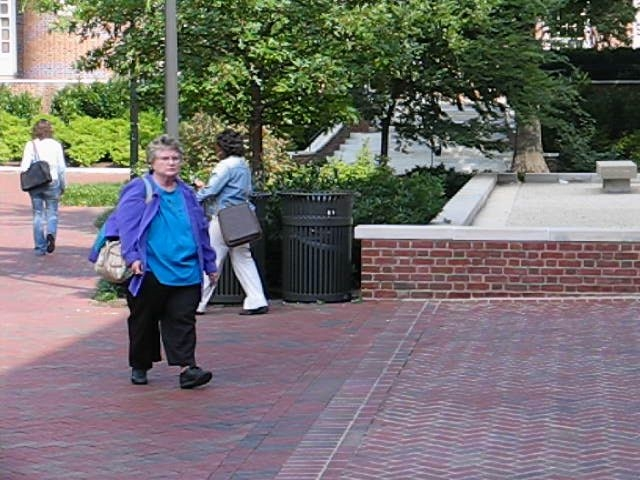
\includegraphics[width=0.22\textwidth]{ch1/in000001.jpg}}%
  \hspace{1em}%
  \subcaptionbox{视频第10帧图像\label{fig:frame10}}
      {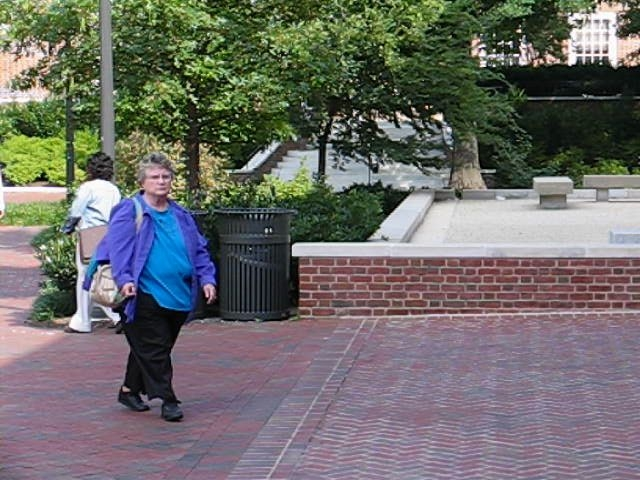
\includegraphics[width=0.22\textwidth]{ch1/in000010.jpg}}
  \hspace{1em}%
  \subcaptionbox{第1帧图像前景\label{fig:frame1Fg}}
      {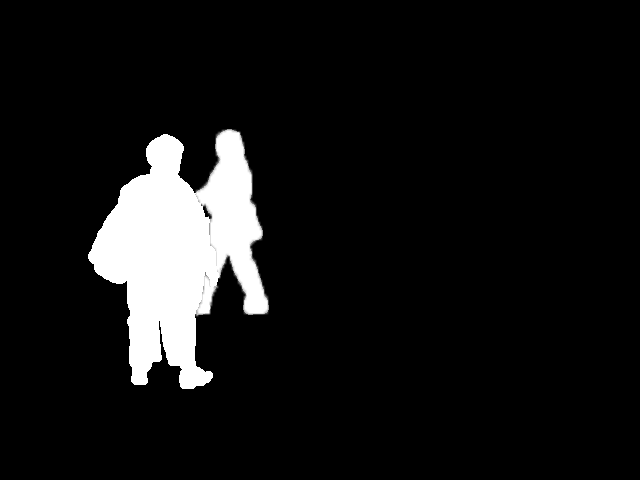
\includegraphics[width=0.22\textwidth]{ch1/gt000001.png}}
   \hspace{1em}%
   \subcaptionbox{第10帧图像前景\label{fig:frame10Fg}}
    {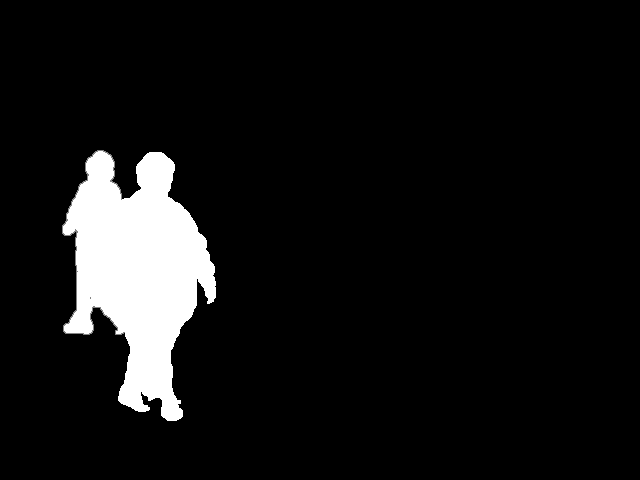
\includegraphics[width=0.22\textwidth]{ch1/gt000010.png}}

  \caption{视频背景减除示例}
  \label{fig:videoBS}
\end{figure}
\par

背景减除通常作为计算机尝试分析并理解图像的第一步,是内容感知的图像处理~\cite{Avidan:2007}、视频监控~\cite{Collins1998A}、目标识别与跟踪~\cite{YilmazTracking}、基于深度的绘制(depth image based rendering,DIBR)~\cite{Fehn03a3d-tv}等应用领域中重要的预处理步骤。例如,在内容感知的图像缩放应用中,为了在对图像进行缩放编辑时保持前景对象的比例,首先需要对图像进行显著性分析,确定显著性对象的位置。在DIBR中,为了处理因遮挡而产生的空洞,需要利用图像中的其它像素对空洞进行填充。因为被遮挡的部分基本上是背景区域,因此如果误将前景像素填充到空洞中,会造成鬼影、闪烁等问题,影响绘制视频的质量。利用背景减除技术对视频进行预处理,可以有效避免将前景像素用于空洞填充,提高视频的绘制质量。\par

综上所述,背景减除技术是计算机视觉研究中一个非常热门的课题。提高背景减除技术的准确度和速度对于众多相关应用具有十分重要的意义。
\section{研究现状}
\label{sec:second}
\subsection{图像显著性分析}
\label{sec:imageSaliency}
图像显著性区域检测的目标是在计算机上实现像人眼一样快速判断图像中显著性区域的能力,通过这种技术提取的图像显著性区域可以广泛用于目标识别,图像编辑以及图像检索等应用。Itti等人~\cite{itti}提出了最早的显著性检测模型,该模型结合了认知心理学,神经科学和计算机科学的理论和方法。基于人类注意力自底向上,关注中心与四周差异的特点,该模型预测人眼观察图像时的焦点,能得到一系列离散的圆点形状的显著性区域预测结果,并不能得到显著性对象的准确边界。随后,显著性检测研究的热点集中在如何获得显著性对象的准确边界,并把它们从图像中分割出来。在这种情况下,显著性检测可以被看作是一个图像分割问题,目标是把图像分割为显著的和非显著的两个部分。如图~\ref{fig:SaliencyOverview}所示,图~\ref{fig:saliencyInput}为输入图像,图~\ref{fig:ITRes}为文献~\inlinecite{itti}所提出算法得到的结果,图~\ref{fig:RCRes}为文献~\inlinecite{ChengPAMI}所提出算法得到的结果,图~\ref{fig:GT}为人工标记的正确结果。

\begin{figure}[ht]
  \centering%
  \begin{subfigure}{0.2\textwidth}
    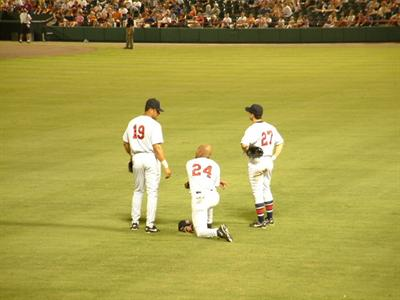
\includegraphics[width=\textwidth]{ch1/0_5_5108.jpg}
    \caption{输入图像}
    \label{fig:saliencyInput}
  \end{subfigure}%
  \hspace{0.1in}%
  \begin{subfigure}{0.2\textwidth}
    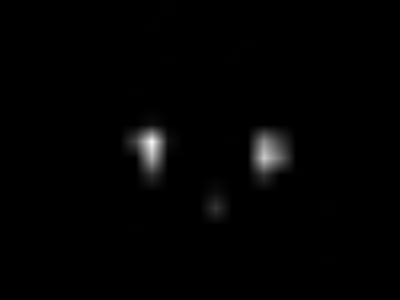
\includegraphics[width=\textwidth]{ch1/0_5_5108_IT.png}
    \caption{~\inlinecite{itti}的结果}
    \label{fig:ITRes}
  \end{subfigure}
  \hspace{0.05in}%
   \begin{subfigure}{0.2\textwidth}
    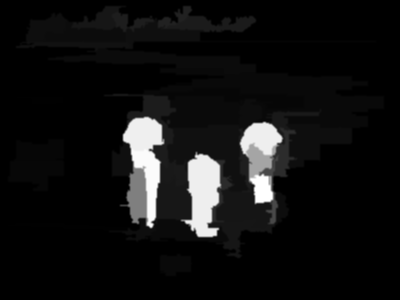
\includegraphics[width=\textwidth]{ch1/0_5_5108_RC.png}
    \caption{~\inlinecite{ChengPAMI}的结果}
    \label{fig:RCRes}
  \end{subfigure}
  \hspace{0.05in}%
   \begin{subfigure}{0.2\textwidth}
    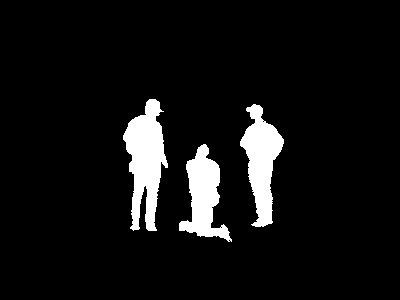
\includegraphics[width=\textwidth]{ch1/0_5_5108.png}
    \caption{正确结果}
    \label{fig:GT}
  \end{subfigure}
  \hspace{0.05in}%
  \caption{显著性分析算法比较}
  \label{fig:SaliencyOverview}
\end{figure}



最近几年以来,显著性区域检测问题一直是计算机视觉等相关研究领域的研究热点~\cite{saliencySurvey}。研究人员提出了一系列新算法,使得显著性对象的准确度以及算法的速度有了显著提高。一般认为,在定位显著性对象时一般依靠内部和外部两种线索\cite{saliencySurvey},其中内部线索来自于待处理图像自身,而外部线索可能来自于用户交互或来自于其它图像的信息。从应用和效率的角度来说,基于内部线索的算法更加贴近实际应用。早期,研究人员关注的内部线索主要是显著性对象的独特性(uniqueness)。这种特性具体表现为,显著性对象与其相邻区域存在较大差异。Achanta等人~\cite{frequenyTuned}提出利用高斯滤波后图像与图像平均颜色差距来计算每个像素的显著性值,图像中像素$x$的显著性指标被定义为:
$$s(x)={\parallel I_{\mu }-I_{\omega}(x)\parallel}^{2}$$
,其中$I_{\mu }$是图像所有像素的平均颜色,$I_{\omega}$是经过高斯滤波后的图像。文献~\inlinecite{patchUniquenss}中提出了一种基于分块独特性(patch uniqueness)的算法,该算法认为图像中那些与最其相似分块的距离大的分块具有较高的显著性水平,并在计算分块显著性时考虑了分块之间的空间距离。Margolin等人~\cite{whatmakes}提出利用分块与图像平均分块的距离来定义分块显著性值,他们认为显著性水平高的分块在高维空间中的分布要更为分散,因此利用分块与平均分块在主元分量方向的距离来定义分块的显著性。\par
然而,基于分块的算法容易使得具有高对比度的图像边缘获得很高的显著性值,而有时这些边缘部分并不是真正的显著性区域。另外,受分块大小参数的影响,这类算法那最终所得的显著性对象的边缘并不准确。基于以上原因,越来越多的显著性分析算法引入了基于区域的分析方法。与基于分块的方法不同,基于区域的方法首先利用区域分割算法对图像进行分割得到若干个齐次的小区域。相比于基于分块以及基于像素的算法, 区域分割处理可以保持对象边界,同时利用区域颜色直方图可以更准确的对区域内的颜色对比度进行量化。另外,以区域为单位计算大大降低了运算量。Cheng等人~\cite{ChengPAMI}提出了一种基于区域对比度的显著性检测算法。该算法首先利用基于图的分割算法~\cite{graphseg}将图像分给为$N$个齐次区域$\{r_{i}\}_{i=1}^{N}$。区域$r_{i}$的显著性值定义为:
$$s(r_{i})=\sum_{j=1}^{N}\omega_{ij}D_{r}(r_{i},r_{j})$$
其中$D_{r}(r_{i},r_{j})$是区域$r_{i},r_{j}$之间的颜色直方图距离,$\omega_{ij}$是区域之间的空间相关性度量。
Perazzi等人~\cite{saliencyFilter}提出利用欧几里得距离来计算$D_{r}(r_{i},r_{j})$,并将显著性计算转换为高斯滤波过程。与文献~\inlinecite{ChengPAMI}中一样,该算法首先将图像进行抽象化(abstraction),去掉不必要的细节部分,将图像分为若干个齐次区域。与文献~\inlinecite{ChengPAMI}中所用的基于图的图像区域分割算法~\cite{graphseg}不同,文献~\inlinecite{saliencyFilter}中使用了边界保持性更好的超像素分割算法~\cite{SLIC}。除了对比度等独特性线索之外,常用的显著性线索还包括中心线索,即图像中显著性对象一般位于图像中靠近中心的位置。此外,文献~\inlinecite{ufo}中提出显著性区域应该在相机的焦点之上,而利用图像中边缘的模糊性可以对图像区域是否在图像焦点上进行量化,综合考虑区域的对比度,和区域中包含对象的可能性(objectness),得到最终显著性结果。\par
与上述基于显著性线索的算法不同,另一类算法从相反的方向考虑问题,利用背景线索来定位背景,最终剩下显著性前景。与显著性对象不同,图像中背景区域具有连续性强;与周围区域相似度高;靠近图像边缘;背景区域之间对比度低等特点。文献~\inlinecite{geodesicDistance}中提出一种基于背景线索的显著性检测算法,该方法利用背景部分像素容易连接到图像边界的特点,利用图像区域距离图像边界的测地线距离(geodesic distance)来评估其显著性。文献~\inlinecite{backgroundPrior}中利用了图像边界大部分是背景这一假设,首先对图像边界区域进行对比度分析,从中获得背景区域主要颜色的线索,之后利用这一线索进行对比度分析获得显著性前景结果。Zhang等人~\cite{zhang2015MBD}提出了一种基于最小障碍距离(minimum barrier distance, MBD)的显著性检测算法,该方法通过评估图像中像素与边界种子点的MBD来计算各像素的显著性值。为了提高效率,文献~\inlinecite{zhang2015MBD}提出基于光栅扫描的MBD近似算法,该算法的计算误差在可接受范围之内,且速度比精确MBD计算算法提高了2个数量级。相比于文献~\inlinecite{geodesicDistance}中的使用的测地线距离,MBD受噪声干扰小且不会产生模糊,因此可以得到更为准确的显著性结果。\par
Hou等人~\cite{SpectralSaliency}提出基于频域分析的显著性区域检测算法, 该算法虽然有处理速度的优势但在准确性上相比于基于空间域的方法还有较大差距。 Huang等人~\cite{Huang2011}提出一种内容感知的随机化图像显著性检测算法,该算法利用多个层次下的粗糙显著性检测结果合成最终结果, 同时选择性的对显著性结果中不可靠的区域进行更新以优化最终结果。此外, 文献~\inlinecite{DISC,NIPS2014_5547}中均提出基于机器学习的图像显著性检测算法。

\subsection{图像填充技术}
\label{sec:imageInpainting}
在图像显著性分析中,一般把显著性对象称为前景对象。这些对象是人眼在观察图像时主要关注的对象。然而在另一种应用场景下,前景和背景需要根据用户的定义来确定,这时原本属于前景的对象可能被用户定义为背景。例如,如图\ref{fig:inpainting}所示,最左边图像中的三棵树原本是前景对象。但因为用户希望获得一幅只有海面和白云的图像而被标记为背景,如图\ref{fig:Inpaint_subfig2}所示,用户希望去掉所标记的对象后得到\ref{fig:Inpaint_subfig3}中的结果。

\begin{figure}[ht]
  \centering%
  \subcaptionbox{输入图像\label{fig:Inpaint_subfig1}}[3cm] %标题的长度,超过则会换行,如下一个小图。
    {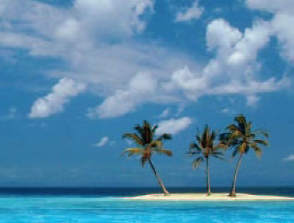
\includegraphics[height=3cm]{ch1/inpaint1.png}}%
  \hspace{4em}%
  \subcaptionbox{红色区域为用户标注的背景\label{fig:Inpaint_subfig2}}
     {
\includegraphics[height=3cm]{ch1/inpaint2.png}}
  \hspace{1em}%
   \subcaptionbox{用户期望的结果\label{fig:Inpaint_subfig3}}
    {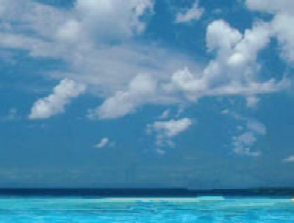
\includegraphics[height=3cm]{ch1/inpaint3.png}}
  \caption{图像修复示例~\cite{Criminisi04regionfilling}}
  \label{fig:inpainting}
\end{figure}

这一应用类型一般被称为图像填充(image inpainting),或图像补全(image completion)。其中用户标注的区域为需要填充的部分,这部分区域根据用户需求而定。在很多情况下包含显著性对象。在填充时,希望能最大限度的保持图像的结构连续性和完整性,使得填充后图像在视觉上没有被修补过的痕迹。图像填充技术在图像编辑、图像去噪、图像编码领域、基于图像的渲染等应用中发挥着重要作用。在我们的日常生活中也经常遇到这样的应用场景,例如在游人如织的旅游景点拍照时会将旁边的路人拍进了画面,这时希望在不破坏原图像的条件下将其从画面中删除;去掉老照片上发黄的部分或者数据丢失后照片中的瑕疵;去掉照片上的文字标题等。\par
假设图像 \emph{I} 中包含未知或缺失部分\(\Omega\) 以及已知区域 \(\overline{\Omega}\),图像填充的目标是利用\(\overline{\Omega}\)中的信息,或者借助来自原图像外部的信息来填充\(\Omega\) 区域。从广义上说,可以把图像填充问题看做是一种特殊的背景减除,需要填充的\(\Omega\)相当于不需要的背景区域,而减除操作相当于用特定像素来填充这些背景区域。图像填充算法大致可以分为两类~\cite{inpaintingSurvey},基于散射(diffusion)的方法~\cite{Bertalmio:2000}和基于样本(examplar)的方法~\cite{Criminisi04regionfilling}。前者利用图像连续和平滑性(smoothness priors)的特点,通过建立参数化的偏微分方程模型方法将已知区域的信息扩散到未知区域。这类方法容易使填充后的图像产生模糊,在缺失区域较大的情况下尤为明显。另一类基于样本的方法则以小图像块为样本,不断将已知区域的结构以及纹理信息传递到位置区域。这类方法不会产生模糊问题,且对图像结构的连续性处理较好。基于样本的方法假设缺失部分的信息可以通过与之最匹配的样本来填充。如图~\ref{fig:examplar}所示,黑色区域为待填充的未知区域\(\Omega\),$\psi_{p}$为以\(\Omega\)的边缘上一点$p$为中心的方块,$\psi_{q}$为\(\overline{\Omega}\)中与$\psi_{p}$最匹配的分块。
\begin{figure}[ht]
  \centering%
      {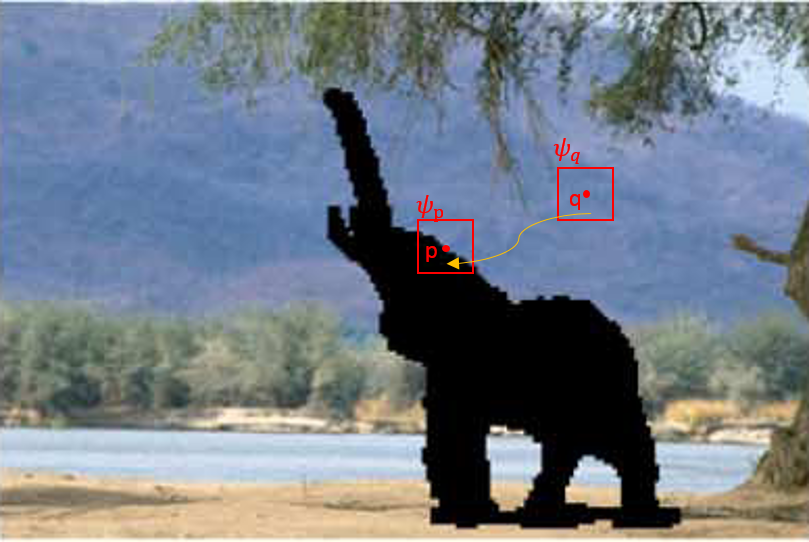
\includegraphics[height=6cm]{ch1/examplar.png}}
  \caption{基于样本的图像修复}
  \label{fig:examplar}
\end{figure}
Efros等人~\cite{Efros}利用$\psi_{q}$的中心点像素来填充$p$,即:
$$Output(p)=Value(q),p\in \Omega, q\in \overline{\Omega},q=\arg \min d(\psi_{p},\psi_{q})$$
,利用分块之间的均方差之和(sum of squared differences,SSD)来计算分块之间的距离,评估分块之间的相似性:
$$d(\psi_{p},\psi_{q})=\sum_{i}^{N}\sum_{j}^{N}\left \| \psi_{p}(i,j)-\psi_{q}(i,j) \right \|^{2}$$
其中$N$为样本的长度和宽度。Criminisi等人~\cite{Criminisi04regionfilling}对Efros等人的算法进行了改进,首先利用未知区域边缘曲线的辐射度方向(isophoto direction)与法向量的夹角来确定分块的填充优先级,使得包含结构信息的分块优先填充,从而保证纹理信息能从已知区域扩散到未知区域;其次,利用最佳匹配块中的对应像素来填充对应未知分块中的像素,比Efros等人的算法效率更高。但是,文献~\inlinecite{Criminisi04regionfilling}提出的算法在一些困难情况下无法恢复未知区域的连续结构信息。文献~\inlinecite{userInpainting}提出了一种用户交互式的基于结构传播的图像补全算法,该方法利用用户输入的一些曲线或者直线把未知区域分为纹理区域和结构区域。对于这两种区域,分别利用不同的策略来恢复纹理信息或结构信息。Xu等人~\cite{Xu:2010}提出另一种基于分块稀疏性(patch sparsity)的图像填充算法,该算法利用分块的稀疏性来确定填充顺序。与之前的方法不同,Xu等人所提算法中并不是只用一个最佳匹配块来对未知区域进行填充,而是利用多个分块的组合来填充未知分块。虽然Xu等人所提算法在填充效果上优于文献~\inlinecite{Criminisi04regionfilling}的算法并且接近基于用户交互的算法~\cite{userInpainting},但是其计算复杂度过高,需要几分钟来处理一张普通大小的图像。Barnes等人~\cite{Barnes:2009}提出一种非常快的随机匹配算法,称为PatchMatch。该方法利用图像的空间相关性,以随机迭代的方式寻找图像的最佳匹配块,并用其进行图像填充。该算法被应用在Adobe公司的Photoshop软件的内容感知填充功能中。虽然PatchMatch算法的速度非常快,处理纹理区域效果好,但是却无法处理包含大块未知结构信息的情况。在这两类算法之外,还有一些算法利用了输入图像之外的信息来进行填充。华淼等提出通过网络检索在互联网或联机数据库中根据输入图像以及所缺失信息进行搜索,寻找合适图像完成输入图像未知区域的填充~\cite{huamiao}。


\subsection{静止相机情况下的视频背景减除}
\label{sec:staticCamera}
在早期的视频背景减除技术研究中,一般假设摄像机是静止的。基于这一假设,通过建立不包含前景对象的背景模型,并将其它图像帧与背景模型进行比较得到前景。
在图~\ref{fig:2}中是一个典型的视频背景减除算法流程图。假设输入视频帧的前$N$帧图像中不包含前景对象,利用这些图像初始化背景模型,在$t$时刻得到的背景模型为$B(t)$。
在下一时刻,将视频图像帧$I(t)$与$B(t)$进行匹配,其中匹配成功的像素标记为背景,反之则为前景。最后利用所得前景结果和当前帧信息对$B(t)$进行更新,得到$B(t+1)$。
由此可见,背景模型的对算法的准确度至关重要。

\begin{figure}[htb]
  \centering%
  {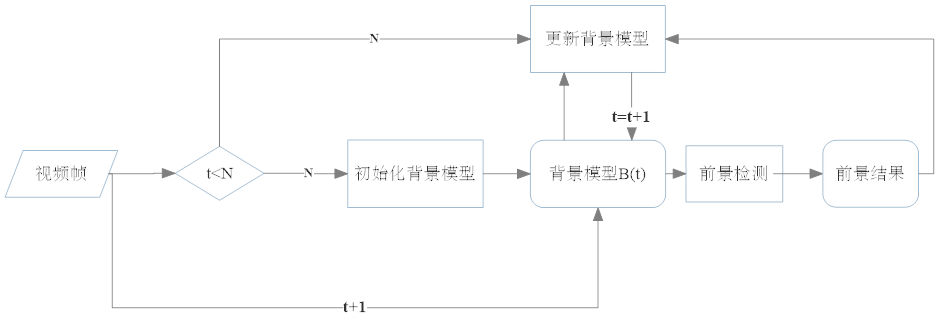
\includegraphics[width=0.9\textwidth]{ch1/bsflowchart.png}}%
  \caption{背景减除流程图~\cite{BouwmansOverview}}
  \label{fig:2}
\end{figure}
最简单的背景模型可以通过对输入视频帧进行平均~\cite{LeeAverage}或者中值滤波~\cite{MF}的方式得到,然而这种方法对噪声的处理并不理想。为了解决这一问题,研究人员提出了一系列基于统计模型的背景建模方法。Chien等人~\cite{Chien2002Efficient}提出了一种基于图像注册背景建模方法,利用一幅图像作为背景模型。该方法首先对视频相邻帧进行
差分操作,并对结果进行二值化得到掩码图像$M$。$M$中值为0的像素为相邻帧图像亮度变化在门限之内的像素,这些像素属于背景的概率较大;然后,观察连续多帧图像产生的$M$,若$M$中某像素长期为0,则其被判为可靠背景像素,并将当期图像帧此位置的像素值复制到背景图像中;最后,将后续的视频帧与背景图像进行差分操作得到前景结果,并对背景图像进行更新。该方法
简单高效,但其依赖固定门限,且仅以一幅图像作为背景模型,无法处理亮度变化大以及包含动态背景的视频。假设视频中像素的亮度值的变化可以用高斯模型来建模,Wren等人~\cite{Wren}提出了单高斯背景模型,随后Kim等人~\cite{kim2007robust}对其进行了改进。然而,这种单高斯模型无法处理像被风吹动的树叶、流动的水等这种动态背景。Stauffer~\cite{stauffer1999adaptive}等人提出了基于自适应混合高斯模型的背景模型建模方法,利用多个高斯模型对背景像素进行建模。相比于单高斯模型,混合高斯模型处理亮度变化大及包含动态背景的视频时效果虽然得到了显著提升,但其前景误检率仍较高。Barnich等人~ \cite{Barnich2011ViBe}提出了一种名为ViBe的无参数采样模型背景建模方法。该方法通过$N$个背景图像色彩空间采样值来描述背景模型:
$$M(x)=\{v_{1},v_{2},...,v_{N}\}$$ \par
如图~\ref{fig:vibe}所示,为了区分某像素$v(x)$是否属于背景,ViBe算法在二维欧几里德色彩空间内计算以$v(x)$为中心的圆形范围$S_{R}(v(x))$内的采样值与背景模型$M(x)$交集的数量,当$\#\{S_{R}(v(x))\bigcap\{v_{1},v_{2},...,v_{N}\} \}$大于或等于某门限值时像素$v(x)$被判为背景,否则为前景。

\begin{figure}[ht]
  \centering%
  {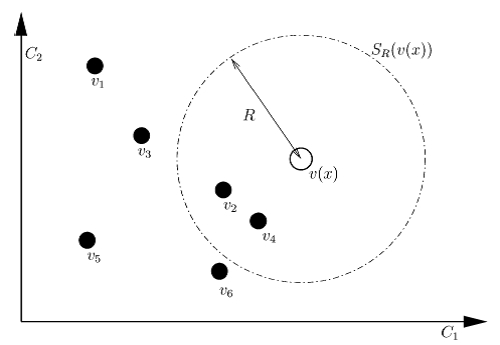
\includegraphics[width=0.5\textwidth]{ch1/vibe.png}}%
  \caption{ViBe算法示意图~\cite{Barnich2011ViBe}}
  \label{fig:vibe}
\end{figure} \par


在背景模型初始化过程中,ViBe算法在第一帧图像中按照均匀分布随机的从像素邻域中选取像素值:${M}^{0}(x)=\{v^{0}(y\mid y\in N_{G}(x))\}$。虽然这种初始化方法可能会将在第一帧中的移动对象设为背景从而产生鬼影现象,但是随着模型的更新,这种现象会逐渐消失。ViBe算法使用一种新的保守的背景更新策略,与之前的更新方法不同的是该算法从背景像素点的历史值中收集样本值,不断更新随机时间序列,当新的样本值加入到背景模型中时随机地将历史样本值丢弃。具体的说,ViBe定义背景模型中的采样值在更新时保留的概率为:
$$P(t,t+dt)={\left(\frac{N-1}{N} \right)}^{(t+dt)-t}$$ \par
另外,为了降低背景更新的频率,ViBe算法还采用时间采样的方式来延长模型的生命周期。若某像素被分类为背景,则以一定的概率(如$\frac{1}{16}$)用该像素的值去更新模型。为了保证空间一致性并使被前景区域覆盖的背景点被更新,在更新时将当前帧$x$点处的像素值去更新在空间八邻域上的邻近像素点的背景模型。ViBe算法简单,鲁棒性强,但也存在一些缺陷:
 \begin{itemize}
\item 当运动目标与背景对比度小的情况下,ViBe 算法提取的目标轮廓存在缺陷,导致目标轮廓不封闭,容易产生轮廓内部孔洞现象;
\item 监控场景下的运动目标有阴影时算法检测出的前景存在阴影现象。
\end{itemize}
\par
Droogenbroeck等人对ViBe算法进行了改进~\cite{vibe},主要修改了距离函数和判别门限,区分更新蒙版和输出蒙版并对其进行了滤波,在更新背景模型时对某些像素进行了限制,当视频中摄像机有抖动时,增大更新系数并检查像素的闪烁。修改后的ViBe算法比原算法普适性更强,并且在检测正确率等方面也有所提高。Hofmann等人~\cite{pbas}提出了一种带反馈的基于像素的自适应视频背景分割算法, 称为PBAS。该方法和ViBe算法一样都是无参数方法。该方法的基本思想和ViBe类似,主要的区别在于PBAS通过自适应的方法对模型更新相关参数进行自适应调整。这种自适应调整通过闭环反馈的方式实现,背景判决门限和更新率等参数可以在处理过程中通过反馈的方式自适应调整,调整后的参数可以获得更好的性能。在测试中PBAS方法的检测准确率等性能参数超过了ViBe,而且同样可以实现实时检测。在近期的一项工作中 \cite{subsenseTIP}, 作者提出了一种更加有效的反馈式模型更新背景建模方法,SuBSENSE. 该算法的准确度在CD.Net 2012~\cite{CDNet2012} 和CD.Net 2014~\cite{CD2014}数据集中均优于其它算法。因为同样是基于采样模型,该算法效率高且易于实现。\par
与上述算法不同,Lin等人~\cite{lin2002a}引入了更复杂的统计模型支持向量机模型(support vector machine,SVM),利用SVM分类器对所有训练视频帧像素进行分类并添加到背景模型,直到不出现新的背景像素时停止模型初始化。SVM所用的特征包括光流信息和图像帧间的差分图像。此外,研究人员还提出了基于子空间学习~\cite{uray2007incremental}和基于频域分析~\cite{Gao2009}的背景模型。文献~\inlinecite{BouwmansOverview}对这些算法进行了总结和分类。

\subsection{移动相机情况下的视频背景减除}
\label{sec:movingCamera}
随着移动计算平台(如智能手机、手持摄像机、智能机器人等)的快速发展, 移动相机视频越来越普及, 针对移动相机拍摄视频的背景减除技术越来越重要。 与静止相机的情况相比, 移动相机下的背景减除要困难很多, 因为相机的运动使得视频中前景和背景像素都会产生运动, 区分相机产生的运动和前景自身运动是待解决的主要难题。另外,如果能利用图像帧准确估算出相机运动,并进行运动补偿,就可以将移动相机情况转换为固定相机情况处理。\par
 文献~\inlinecite{iccv2009}提出一种基于点轨迹的背景减除算法, 根据背景点轨迹矩阵的秩等于3的特点~\cite{Tomasi_1992}, 以滑动窗口的方式利用随机抽样一致(random sample consensus, RANSAC) 算法~\cite{Ransac} 在点轨迹矩阵中检测背景点。 同样基于点轨迹并考虑前景像素的集中性, 文献~\cite{Cui2012}提出一种基于点轨迹矩阵分解的算法。Berger等~\cite{SubspaceTracking}提出一种基于线性子空间跟踪的背景建模算法, 与基于点轨迹的同类算法相比, 该算法的背景检测更准确, 且处理速度更快, 但其处理一帧图像仍需要1.6秒。 另外, 由于这类算法是基于点轨迹的, 而计算视频中稠密像素的长期轨迹是一项十分耗时且困难的工作, 即使在GPU 加速的情况下也需要几秒的时间处理一帧图像~\cite{ECCV10DensePonintTrajectories}。\par

为了处理相机的运动, 另一类算法引入了稠密光流。 文献~\inlinecite{kwak2011Generalized}提出一种基于贝叶斯滤波的背景减除算法框架, 该算法需要视频第一帧的准确前景作为输入, 并在随后的视频帧中利用稠密光流信息进行可靠跟踪; 这种算法需要人工交互来生成第一帧的准确前景, 不适用于在线处理, 且无法处理长时间且包含复杂相机运动的视频. 文献~\inlinecite{gbsuperpixel}提出另外一种基于稠密光流的移动相机视频背景减除新算法, 通过建立基于超像素的背景模型, 并基于二进制置信传播技术通过多次迭代获得像素级精度的前景; 虽然该算法的准确度要优于其他算法, 但其处理一帧大小为$300\times200$的视频帧需要6秒。\par
文献~\inlinecite{5.8s}提出一种实时的移动相机下视频背景减除算法, 由于该算法利用基于固定特征点跟踪的相机运动估算算法和简化的双模高斯背景模型, 使得算法复杂度低速度较快, 并可以实现实时处理。但文献~\inlinecite{5.8s}没有给出该算法前景检测准确度的定量分析。 本文通过实验发现, 文献~\inlinecite{5.8s}算法的前景检测准确度较低, 特别是在相机移动幅度较大的情况下, 无法适应前景检测准确率要求较高的应用。\par
在估算相机运动,一般采用单应性矩阵或基础矩阵来描述相机运动情况。 文献~\inlinecite{Multitransform}中提出了一种多变换模型的方法来处理相机运动。该算法根据相邻帧图像的几何变换情况,自适应地从单应性矩阵模型和基础矩阵模型中选择一个模型。当选择单应性矩阵时,根据特征点的运动情况估算全局单应性矩阵并用于相机运动补偿,而当选择基础模型使用时,基于最小均方误差的方式在一系列单应性矩阵中选择一个误差最小的单应性矩阵作为全局参数补偿相机运动。\par
崔智高等~\cite{czg}提出一种基于多组单应约束和马尔可夫随机场(Markov random field,MRF)的移动目标检测算法, 通过轨迹分离和像素标记2个阶段实现移动相机拍摄视频中运动目标的检测; 该算法检测前景的准确度较高, 但由于算法是基于点轨迹的, 同样存在算法计算量大的问题。



\section{研究目标与主要贡献}
\label{sec:contents}
快速识别图像和视频中的显著性前景,将前景对象从背景中分离出来是人类的视觉系统与生俱来的能力。然而,在计算机上实现人眼的这种能力却十分困难。对于图像显著性检测,主要的困难在于:
 \begin{itemize}
     \item 前景的多样性和不确定性。相比于人脸识别、指纹识别等应用,显著性检测的目标并不固定。在不同的场景下,前景对象的定义存在不确定性,例如,在一张汽车广告画中汽车是前景对象,然而同样是汽车, 在车模的特写照片中却成为背景;
	\item 复杂背景情况。当图像中的背景较复杂时,会使得背景部分的像素也具有对比度高、独特性明显等性质,而这些指标常用于检测显著性对象,这时容易将背景误识别为前景,造成误检率高。
\end{itemize}
当前视频背景减除面临的主要困难主要有:
\begin{itemize}
	\item 噪声干扰。在环境噪声的干扰下,我们得到的视频图像中可能包含一些噪声,这些噪声会对前景提取的准确度造成重要的影响。例如在雨雪天气或者夜间拍摄的视频中,存在亮度不足,雨雪对前景判别产生干扰等问题;
    \item 动态背景,在视频背景减除中,我们在判别前景和背景时一般假设背景区域的像素是静止,而运动的像素则属于前景。然而,在实际应用中,这一假设并不总是成立。例如视频中被风吹动摇摆的树叶,喷泉,以及流动的水面等。这些对象虽然是运动的,但实际却属于背景;
    \item 相机的运动,在早期的视频背景减除技术研究中,一般假设相机是静止的。然而,随着移动计算平台,例如手机、手持摄像机、智能机器人等的出现,移动相机拍摄视频中的背景减除技术研究越来越重要。在移动相机拍摄的视频中,区分相机运动和前景运动是一项困难的工作。
  \end{itemize}

\par
在图像填充技术方面,主要的困难在于保持图像结构信息的连续性,此外当前效果较好的算法速度较慢,处理一张普通大小的图像可能要几分钟时间,很难满足人们在线处理的应用需求。针对上述这些问题,本论文围绕图像和视频中的背景减除技术展开研究,主要研究目标是提出更加高效且准确的方法来提取图像和视频中的显著性前景。本论文主要研究内容为图像显著性检测、图像填充以及针对移动相机拍摄视频的背景减除,主要贡献总结如下:
 \begin{itemize}
    \item 将图像显著性区域检测问题视为图像分割问题,提出以显著性引导的区域合并的方式将图像分为显著性区域(前景)和背景两个区域。在合并过程中采用了与主流算法相反的策略,即不再尝试定位显著性区域,而是利用背景线索来估计背景区域,并不断将显著性差的非前景区域合并到背景区域。利用背景连续性强、靠近图像边缘、相对前景对比度低等背景线索,首先将图像进行超像素分割,随后在区域显著分析的引导下,不断将显著性最差的区域合并到背景区域,而不是尝试将显著性区域合并到一起。 最后,利用合并过程中得到的多个候选显著性区域加权得到最终的显著性区域结果。在国际上两个公开的数据库中的共计2000张图像上对本文所提出的算法进行了测试,实验结果验证了算法的有效性。在主要由自然图片组成,较为困难的ECSSD~\cite{ECSSD}测试集中,本文算法得到的F-Mearsure以及平均绝对误差(mean absolute error,MAE)均优于其它同类算法。此外,本文的算法简单直观,且效率高、易于实现;
    \item 针对现有的基于样本的图像填充算法容易造成结构信息不连续且计算量大的问题,提出了一种基于样本的两阶段快速图像填充算法,以两次填充的方式将结构以及纹理信息填充到图像中的未知区域中。该算法首先利用离散小波变换(discrete wavelet transform, DWT)获取低分辨率的输入图像,并利用基于样本的填充算法进行填充。由于高频细节部分被DWT过滤,在低分辨率填充后的图像中纹理部分区域可以获得较好的结果,但是在包含边缘的局部还存在着结构不连续的情况。针对这些问题,在这些区域中再进行第二次填充。在填充过程中,提出基于梯度结构张量的填充优先级计算方法以及基于加权SSD的最佳匹配块标准以提高填充后图像的结构和纹理连续性。为了提高效率,提出了以分块结构性测试和动态搜索窗口的方式寻找最佳匹配分块,减少冗余计算。本文提出的填充算法可以得到与当前先进算法相近的结果,但是在处理速度上却有明显优势;
    \item 提出了一种基于无参数模型的快速视频背景减除算法。该算法利用两种线索来有效检测移动相机拍摄视频中的前景对象。第一种线索基于色彩空间和纹理特征空间采样模型,通过引入最相似变形(as-similar-as-possible warping, ASAPW)方法来准确估算相机运动并进行补偿,然后将变形后的图像与背景模型进行匹配得到一张粗略的前景分割图像;第二种线索来基于前景引起的运动与相机引起的运动的差异。利用稀疏光流和相机运动的差异获取背景种子点,提出一种基于超像素种子点的区域增长算法,将稀疏的背景种子点扩散到整张图像,获得另一张粗略的前景图;最后为了融合两种线索的结果并考虑时间上的相关性,提出了一种基于超像素的MRF优化框架,将两种线索得到的粗略前景以及上一帧图像所得的前景结果值一起输入优化方法,最后通过图割算法求解得到最终结果;
    \item 提出了一种针对移动相机的实时背景减除算法。该算法假设视频中大部分区域是背景, 前景只占相对较小部分。考虑背景像素的连续性, 提出了一种基于超像素的区域增长算法对图像进行预处理。 为了估算相机运动, 提出了一种基于相对光流的特征点筛选算法, 筛选出属于背景的特征点, 并利用这些特征点以分块的方式估算相机的运动。 最后通过比较这些超像素的光流与所估算的相机运动的一致性来确定最终的前景。该算法简单直接, 不需要建立任何背景模型, 利用GPU和CPU的混合编程可以实现实时处理。 大量实验证明该算法的前景检测准确度远高于同类实时算法。
  \end{itemize}
\section{本文的组织结构}
\label{sec:hierarchy}
本文第一章为引言,介绍了论文的研究背景和意义,并对国内外相关工作进行了综述,最后介绍了本文的研究内容以及主要贡献。第二章研究图像显著性检测问题,介绍了本文提出的基于区域合并的图像显著性检测算法,第三章中介绍本文提出的基于样本的快速图像填充算法,第四章和第五章研究移动相机情况下的视频背景减除问题,第四章中介绍了本文提出的基于无参数模型的快速背景减除算法,第五章介绍了本文提出的另一种简单有效的实时背景减除算法。第六章对全文进行了总结和展望。
